\section{Selection}
\label{sec:analysis:selection}


% ===========================
% Object Selection
% ===========================

\subsection{Object Selection}
The event topologies of interest will require reconstructing electrons, muons, hadronically decaying tau leptons, hadronic jets, and missing tansverse energy (MET).  In this section, the reconstruction and selection of these physics objects is described.



\subsubsection{Primary vertex}
Primary vertices (PV) are reconstructed based on information from the tracking subsystem, mainly through the inner pixel detector. Quality cuts are applied to reconstructed PVs to guarantee they come from a proton-proton hard scattering event. These cuts are as follows,
\begin{itemize}
    \item $N_{d.o.f.}> 4$;
    \item $\left|z\right| < 24~\mathrm{cm}$; 
    \item $\sqrt{x^{2} + y^{2}} < 2~\mathrm{cm}$.
\end{itemize}
The PVs are ordered based on the sum \pt of tracks used in their reconstruction.  Selected physics objects are associated to the PV with the greatest sum \pt. 




\subsubsection{Muon}
Muon candidates are reconstructed using both the muon and tracker systems. The coverage of these two detector systems allows reconstruction of muons within $\left|\eta\right| < 2.4$ and $p_{T}$ as low as 5 GeV~\cite{Chatrchyan:2012xi}. 

Muons are required to be reconstructed using both the \emph{global muon} and \emph{tracker muon} reconstruction algorithms.  These algorithms are distinct in that one begins with tracker information and extrapolates to find consistency with hits in the muons system (\emph{tracker muons}), while the other (\emph{global muon}) inverts the reconstruction steps starting from the muon system and finding tracks that are consistent. The combination of these two algorithms makes for a muon reconstruction that is accurate in predicting muon momentum and efficient in detecting muons within the detector acceptance.

In the interest of detecting muons decaying from vector bosons, a set of identification and isolation requirements are applied~\cite{Sirunyan:2018fpa}. The muon identification requirements are designed to have high selection efficiency and a low probability of misidentifying nonprompt muons originating from non-bosonic decays. The muon POG provided selection criteria are listed in table~\ref{tab:muon_id}.

\begin{table}[ht]
    \centering
    \setlength{\tabcolsep}{2em}
    \renewcommand{\arraystretch}{1.25}
    % \small
    \caption{Tight muon identification criteria as provided by muon POG}
    \label{tab:muon_id}
    \begin{tabular}{l|c}
    variable                            & cut value \\
    \hline
    isGlobal                            & True      \\
    isPF                                & True      \\
    $\chi^{2}$                          & $< 10$    \\
    number of matched stations          & $> 1$     \\
    number of pixel hits                & $> 0$     \\
    number of track layers              & $> 5$     \\
    number of valid hits                & $> 0$     \\
    $|d_{xy}|$                          & $< 0.2$   \\
    $|d_{z}|$                           & $< 0.5$    \\
    \hline
    $ISO_{PF}/p_{T}$ ($\rho$ corrected) & $< 0.15$
    \end{tabular}
\end{table}


\noindent To increase the likelihood of selecting muons produced by the prompt decay of vector bosons, an isolation requirement is placed on all muons. The isolation of the muon is calculated by summing the \pt of all charged hadronic, neutral hadronic, and photon particle flow candidates in a cone of radius $\Delta R = 0.4$ about the muon candidate. This quantity is corrected to remove the contamination of the neutral component due to pileup by subtracting off the average energy deposited by pileup. It is defined as,

\begin{equation}
    ISO_{PF} = Iso_{\rm ch. had} + max \left(0, Iso_{\rm neu. had} +
    Iso_{\gamma} - 0.5 Iso_{\rm pileup}\right)
\end{equation}

Simulated events are reweighted to account for differences in the muon reconstruction, identification, and isolation efficiencies with respect to data.







\subsubsection{Electron}

Electrons are reconstructed by combining information from the electromagnetic calorimeter and the tracking system using a gaussian-sum
filter (GSF) method \cite{Baffioni:2006cd}.  Corrections are applied to account for mismeasurement of electron momentum scale and resolution. All electrons are required to have $\pt \geq 20~\GeV$ and $|\eta| < 2.5$.  Electrons are identified using a tight cut-based scheme. The requirements for this selection are listed in table~\ref{tab:slt:electron_id}.

\begin{table}[ht]
    \centering
    \setlength{\tabcolsep}{2em}
    \renewcommand{\arraystretch}{1.25}
    % \small
    \caption{Tight electron identification criteria as provided by the egamma POG.}
    \label{tab:slt:electron_id}

    \begin{tabular}{l|c|c}
        variable                          & $|\eta| < 1.4446$ & $|\eta| \geq 1.566$ \\
        \hline
        $\sigma_{i\eta}\sigma_{i\eta}$    & $<0.00998$        & $0.0394$            \\
        $|d\eta|$                         & $<0.00308$        & $0.0292$            \\
        $|d\phi|$                         & $<0.0816$         & $0.00605$           \\
        $H/E$                             & $<0.0414$         & $0.0641$            \\
        $|\frac{1}{E} - \frac{1}{p}|$     & $<0.0129$         & $0.0129$            \\
        missing hits                      & $\leq 1$          & $\leq 1$            \\
        $|d_{0}|$                         & $<1.$             & $<1.$               \\
        \hline
        conversion rejection              & true              & true                \\
        ISO$_{PF}$/$p_{T}$ (EA corrected) & $< 0.0588$        & $<0.0571$           \\
    \end{tabular}
\end{table}

\noindent The electrons are also required to pass a tight isolation criteria. The isolation variable is constructed by summing the energy of charged and neutral particle flow objects within a cone of radius $\Delta R = 0.4$ about the electron candidate and subtracting off the contribution from pileup.  The combined particle flow isolation with the pileup correction is,

\begin{equation}
    \nonumber
    Iso_{comb} = Iso_{\sf ch. had.} + max\left(0, Iso_{neu. had.} + Iso_{\gamma} - \rho EA(|\eta_{e}|) \right).
\end{equation}

The pileup correction is dependent on the parameter $\rho$ which correlates with the average energy due to pileup, and the effective area which changes depending on the $|\eta|$ value of the electron.





\subsubsection{Hadronic Tau}

Hadronically decaying $\tau$ leptons are reconstructed using the hadron-plus-strips algorithm~\cite{ref:cms-tau}. This algorithm constructs candidates seeded by a PF jet that are consistent with either a single or triple charged pion decay of the $\tau$ lepton.  In the single charged pion decay mode, the presence of neutral pions is detected by reconstructing their photonic decays.  If the hadronic tau candidate is found to overlap ($\Delta R < 0.3$) with either an electron or muon passing the analysis selections listed above, the tau candidate is rejected.  Jets originating from non-$\tau$ decays are rejected with a MVA discriminator that takes into account the pileup contribution to the neutral component of the $\tau$ decay~\cite{CMS-TAU-16-003-001}.  

Reconstructed hadronic taus are required to have $p_{T} > 20$ GeV and $|\eta| < 2.3$ unless noted otherwise.  It is observed that the counting analysis is more sensitive to misidentification of hadronic jets as hadronic tau candidates, so while the tight working point is used in the shape analysis, the very tight working point is used for the counting analysis.

The scale factor accounting for different tau reconstruction and identification efficiencies were measured in several control regions~\cite{CMS-TAU-16-003-001}.  The measurement is carried out in both in two different control regions: one enriched in $\PZ\to\tau\tau$ production and one enriched in \ttbar.  Because of the large overlap with our signal region in the case of the latter, the former measurement is used so that the datasets that are used are uncorrelated.  For the selection algorithm and tight working point a scale factor of $0.95 \pm 0.05$ is used; for the very tight working point it is $0.92 \pm 0.05$.






\subsubsection{Jet}
Jets are reconstructed from PF candidates \cite{ref:pf}. PF candidates combine information from all of the detector subsystems to facilitate the reconstruction and identification of individual particles.  These PF candidates are clustered using the anti-$k_{t}$ algorigthm \cite{Cacciari:2008gp} with a cone size of $\Delta R = 0.4$. Once reconstructed, a number of corrections are applied to the jets to correct for pileup contamination, differing absolute response in jet \pt, and relative response in $\eta$ \cite{ref:jetscale}.  To reduce contamination from photons and prompt leptons, several ID requirements are placed on the jets and are listed in table~\ref{tab:slt:jet_id_2016}.

\begin{table}[ht]
    \centering
    \setlength{\tabcolsep}{0.8em}
    \renewcommand{\arraystretch}{1.25}
    % \small
    \caption{Jet ID requirements for 2016.}
    \label{tab:slt:jet_id_2016}
    \begin{tabular}{l|ccc}
        \hline
                                    & $|\eta| < 2.4$ & $2.4 < |\eta| \leq 3.0$ & $3.0 < |\eta| \leq 4.7$ \\
        \hline                                                                   
        number of constituents         & $> 1$          & $> 1$                  & -- \\
        neutral hadronic fraction      & $< 0.99$       & $< 0.99$               & -- \\
        neutral EM fraction            & $< 0.99$       & $< 0.99$               & $<0.9$ \\
        charged hadronic fraction      & $> 0$          & --                     & -- \\
        charged EM fraction            & $< 0.99$       & --                     & -- \\
        number of charged constituents & $> 0$          & --                     & -- \\
        number of neutrals             & --             & --                     & $>10$                   \\
        \hline
    \end{tabular}
\end{table}

\noindent In addition to the above requirements, it is required that all jets have $\pt > 30$ GeV and $\left|\eta\right| < 4.7$.  Jets are vetoed if they overlap with a muon, electron, or tau passing the identification requirements described above within a cone size of $\Delta R = 0.3$. 

The identification of jets originating from the decay of b quarks is done using the CSV b-tagging algorithm~\cite{Sirunyan:2298594} is used to optimize the efficiency for identifying b-jets while reducing the misidentification from jets originating from light quark (usdg).  In this analysis, the recommended medium working point ($\text{CSV} > 0.8484$) supplied by the b tag POG is used.  

To account for the difference in b tag efficiency in data and simulation, the b tag status of jets is modified based on a set of scale factors derived by the b tag POG.  The method used for applying the b tag scale factors modifies the status of individual jets to either promote or demote their b tagging status~\cite{twiki:btag_method}.  The method relies on the user measuring the b tag and mistag efficiencies in the simulated samples.  This is described further in appendix~\label{app:btag}.


\FloatBarrier

% ===========================
% Event Selection
% ===========================
\subsection{Event Selection}

The event selection begins by requiring an event pass the lowest \pt theshold single electron or muon trigger that is not prescaled. From these datasets it is possible to select on a number of $\PW\PW$-like final states originating from \ttbar and tW production.  These final states are constructed based on the number of reconstructed leptons, jet multiplicity, and b tag multiplicity.  The categorization of these events differs between the counting and shape analysis.  The common definition of the categories are listed below.


\begin{table}[ht]
	\centering
	\setlength{\tabcolsep}{0.4em}
    \renewcommand{\arraystretch}{1.5}
    \small
    
    \begin{tabular}{|cc|cc|cc|cc|}
    
    %%%%%%%%%%%%%%%%%%
	% mu-trigger
	%%%%%%%%%%%%%%%%%%
    \multicolumn{8}{c}{single muon trigger} \\
    \hline
    \multicolumn{2}{|c|}{$\mu e$} 					& \multicolumn{2}{c|}{$\mu\mu$} 				  & \multicolumn{2}{c|}{$\mu \tau$} 					& \multicolumn{2}{c|}{$\mu + jets$} 			  	\\
    \hline
    1b & 2b                   						& 1b & 2b        	 						      & 1b & 2b        										& 1b & 2b         			        				\\
    \hline 
    \multicolumn{2}{|c|}{$n_{e,\mu,\tau_h} = 1,1,0$}& \multicolumn{2}{c|}{$n_{e,\mu,\tau_h} = 0,2,0$} & \multicolumn{2}{c|}{$n_{e,\mu,\tau_h} = 0,1,1$}      & \multicolumn{2}{c|}{$n_{e,\mu,\tau_h} = 0,1,0$} 	\\
    \multicolumn{2}{|c|}{$p^T_\mu,p^T_e>25,15$ GeV} & \multicolumn{2}{c|}{$p^T_\mu,p^T_\mu>25,10$ GeV}& \multicolumn{2}{c|}{$p^T_\mu,p^T_{\tau_h}>30,20$ GeV}& \multicolumn{2}{c|}{$p^T_\mu>30$ GeV}           	\\
    \multicolumn{2}{|c|}{$p^T_\mu>p^T_e$} 			& \multicolumn{2}{c|}{$|m_{\mu\mu}-m_Z|>15$ GeV } & \multicolumn{2}{c|}{ --- }						     & \multicolumn{2}{c|}{ --- } 						\\
    \multicolumn{2}{|c|}{$n_{jet}\geq2$}			& \multicolumn{2}{c|}{$n_{jet}\geq2$}             &  \multicolumn{2}{c|}{$n_{jet}\geq2$} 				 & \multicolumn{2}{c|}{$n_{jet}\geq4$}             	\\
    \hline

    
    %\multicolumn{8}{c}{} \\
    \multicolumn{8}{c}{single electron trigger} \\
    
    %%%%%%%%%%%%%%%%%%
	% e-trigger
	%%%%%%%%%%%%%%%%%%
    \hline
    \multicolumn{2}{|c|}{$e e$} 					& \multicolumn{2}{c|}{$e \mu$} 				      & \multicolumn{2}{c|}{$e \tau$} 			     		& \multicolumn{2}{c|}{$e + jets$} 			     	\\
    \hline
    1b & 2b                   						& 1b & 2b        	 						      & 1b & 2b        										& 1b & 2b         			        				\\
    \hline 
    \multicolumn{2}{|c|}{$n_{e,\mu,\tau_h} = 2,0,0$}& \multicolumn{2}{c|}{$n_{e,\mu,\tau_h} = 1,1,0$} & \multicolumn{2}{c|}{$n_{e,\mu,\tau_h} = 1,0,1$}      & \multicolumn{2}{c|}{$n_{e,\mu,\tau_h} = 1,0,0$} 	\\
    \multicolumn{2}{|c|}{$p^T_e,p^T_e>30,15$ GeV}   & \multicolumn{2}{c|}{$p^T_e,p^T_\mu>30,10$ GeV}  & \multicolumn{2}{c|}{$p^T_e,p^T_{\tau_h}>30,20$ GeV}  & \multicolumn{2}{c|}{$p^T_e>30$ GeV}           	\\
    \multicolumn{2}{|c|}{$|m_{ee}-m_Z|>15$ GeV }    & \multicolumn{2}{c|}{$p^T_e>p^T_\mu$}   		  & \multicolumn{2}{c|}{ --- }						     & \multicolumn{2}{c|}{ --- } 						\\
    \multicolumn{2}{|c|}{$n_{jet}\geq2$}			& \multicolumn{2}{c|}{$n_{jet}\geq2$}             & \multicolumn{2}{c|}{$n_{jet}\geq2$} 				 & \multicolumn{2}{c|}{$n_{jet}\geq4$}             	\\
    \hline
    
    \end{tabular}
    
    \caption{Analysis selections of 8 channels based on single muon and single electron triggers.}
    \label{tab:slt:eventSelection}
\end{table}

These selections are designed to primarily target $\ttbar$ production and specific \PW decay modes.  The final states will tend to only contain events from a single datastream except for the $e\mu$ selection which has non-negligible overlap between the electron and muon datastreams.  Any overlap in events between the two datastreams are removed by only taking the event from single muon datastream.  Because the tau can decay to an electron, muon, or hadronically, each of these channels has some mixing between terms arising from $W\rightarrow\ell$ decays and $W\rightarrow\tau\rightarrow\ell$ decays.  The mixing between the selected final states and the underlying W boson decays are shown in table~\ref{sigcomp}.  These numbers are estimated from simulated \ttbar events and are consequently dependent on the values of branching fractions used in the simulation.  


\begin{figure}[ht]
    \centering
    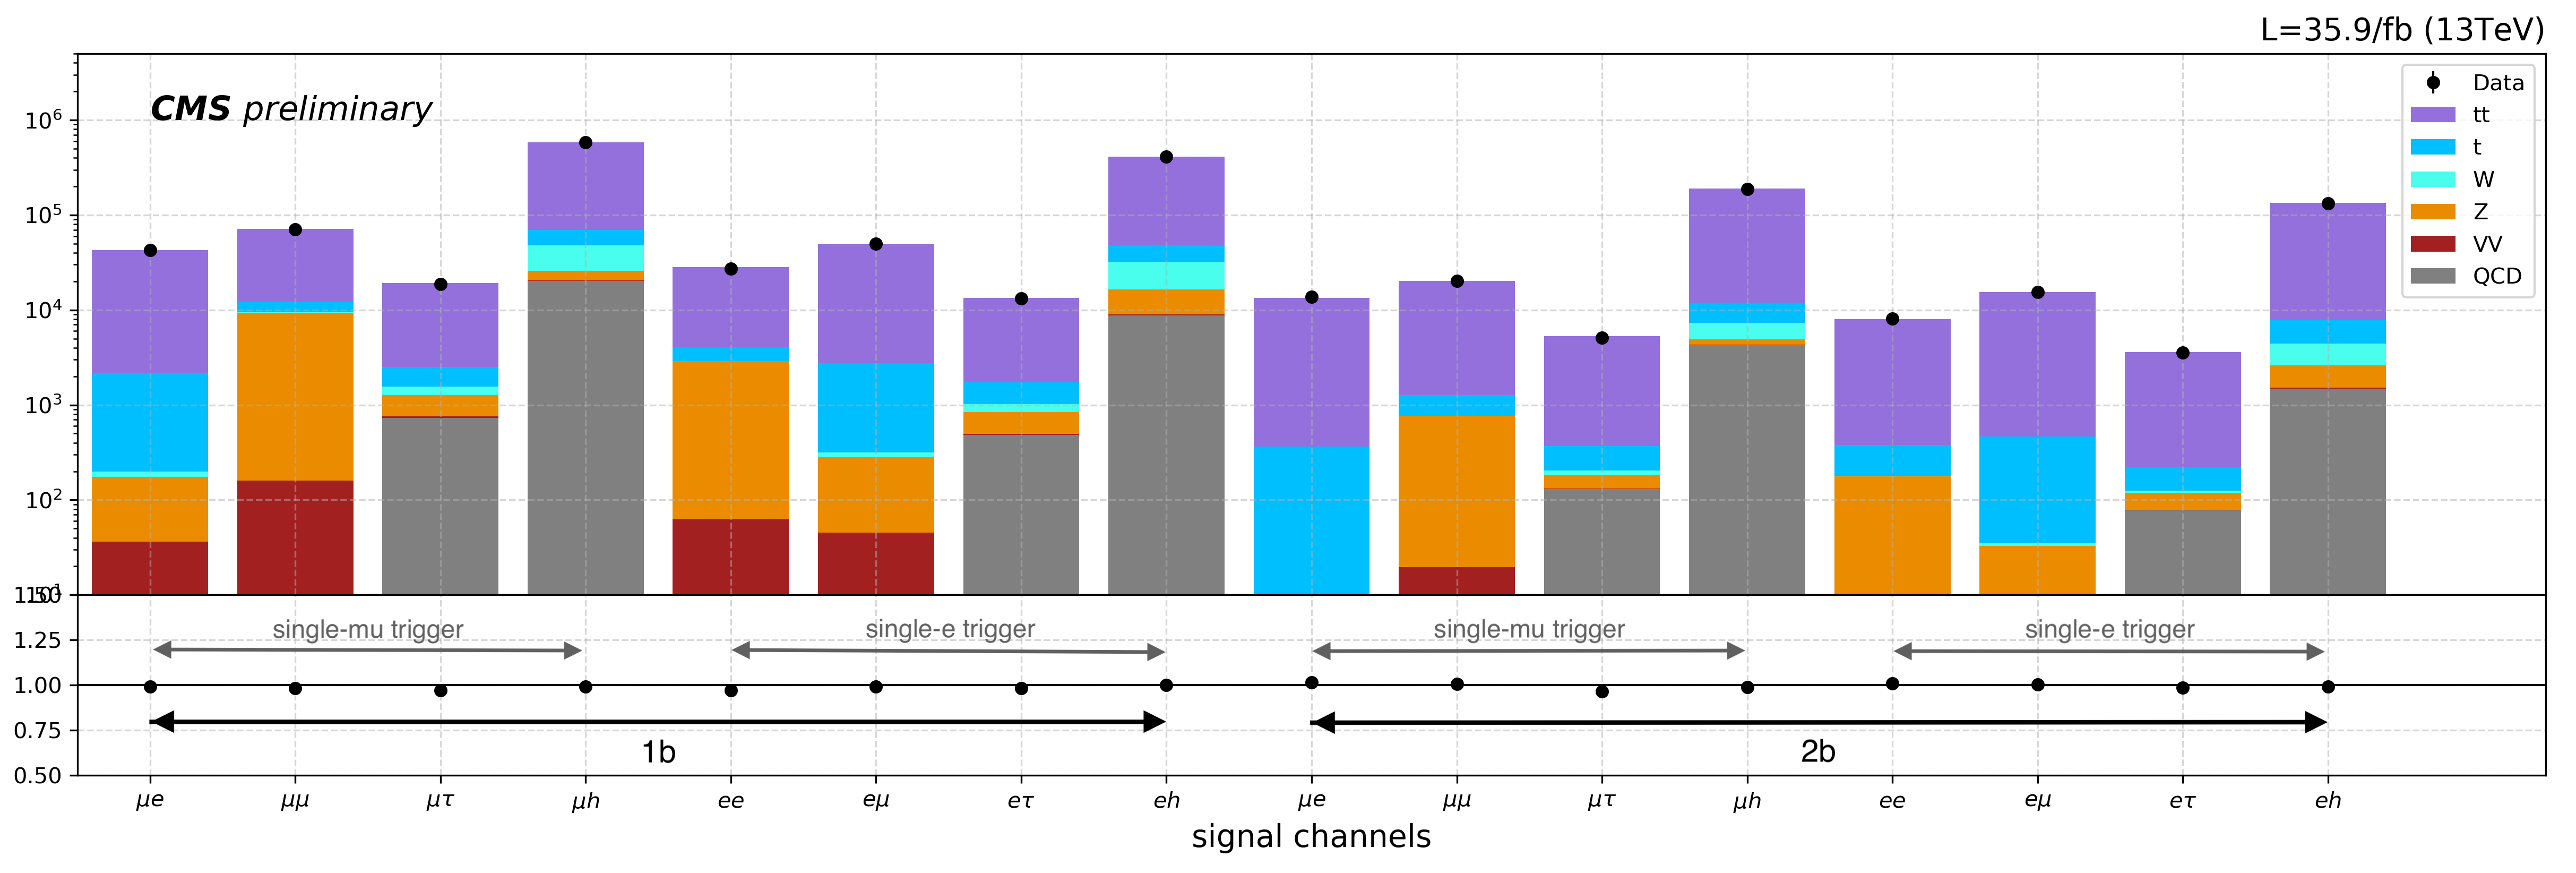
\includegraphics[width=0.99\textwidth]{chapters/Analysis/sectionSelection/figures/counting.png}
    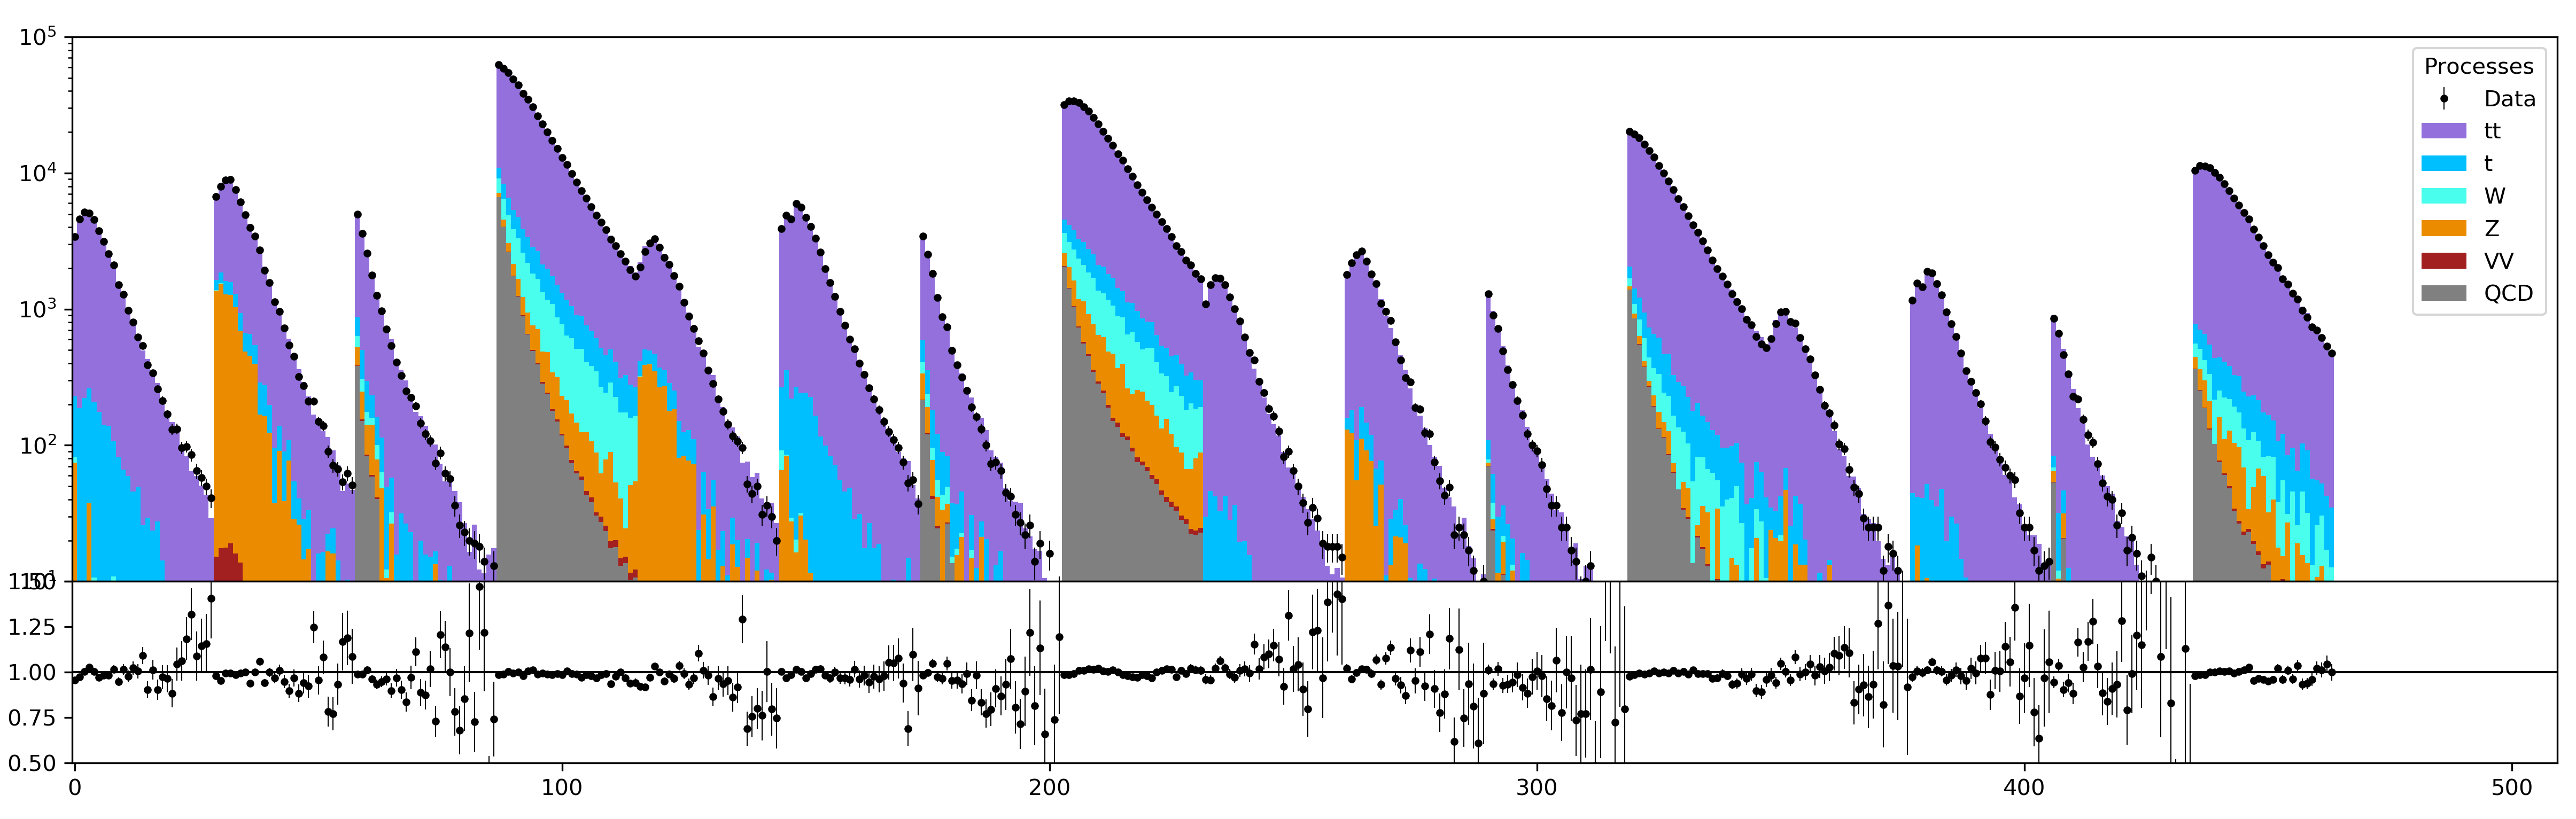
\includegraphics[width=0.99\textwidth]{chapters/Analysis/sectionSelection/figures/shaping.png}
    \caption{caption}
    \label{fig:analysis:selection:yields}
\end{figure}


\begin{figure}[ht]
    \centering
    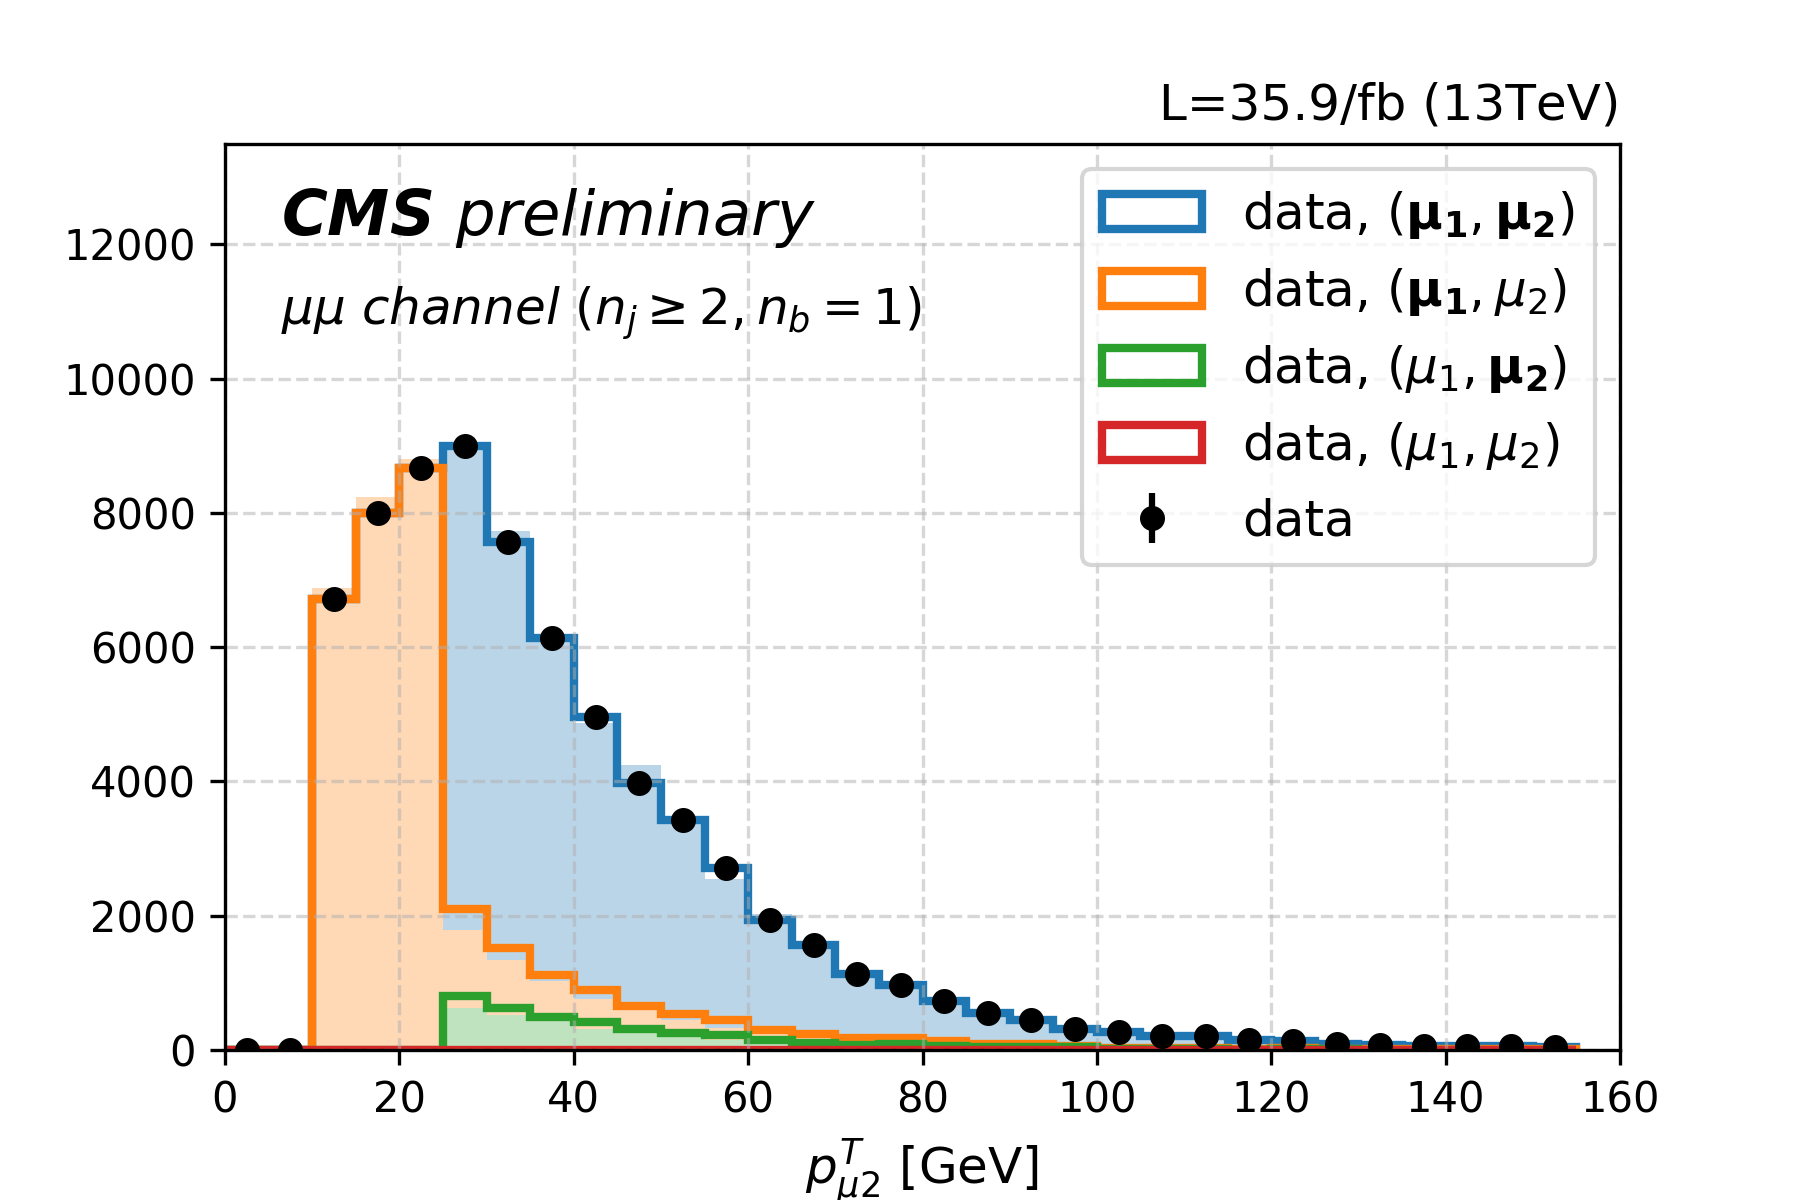
\includegraphics[width=0.49\textwidth]{chapters/Analysis/sectionSelection/figures/trgLep_mumu.png}
    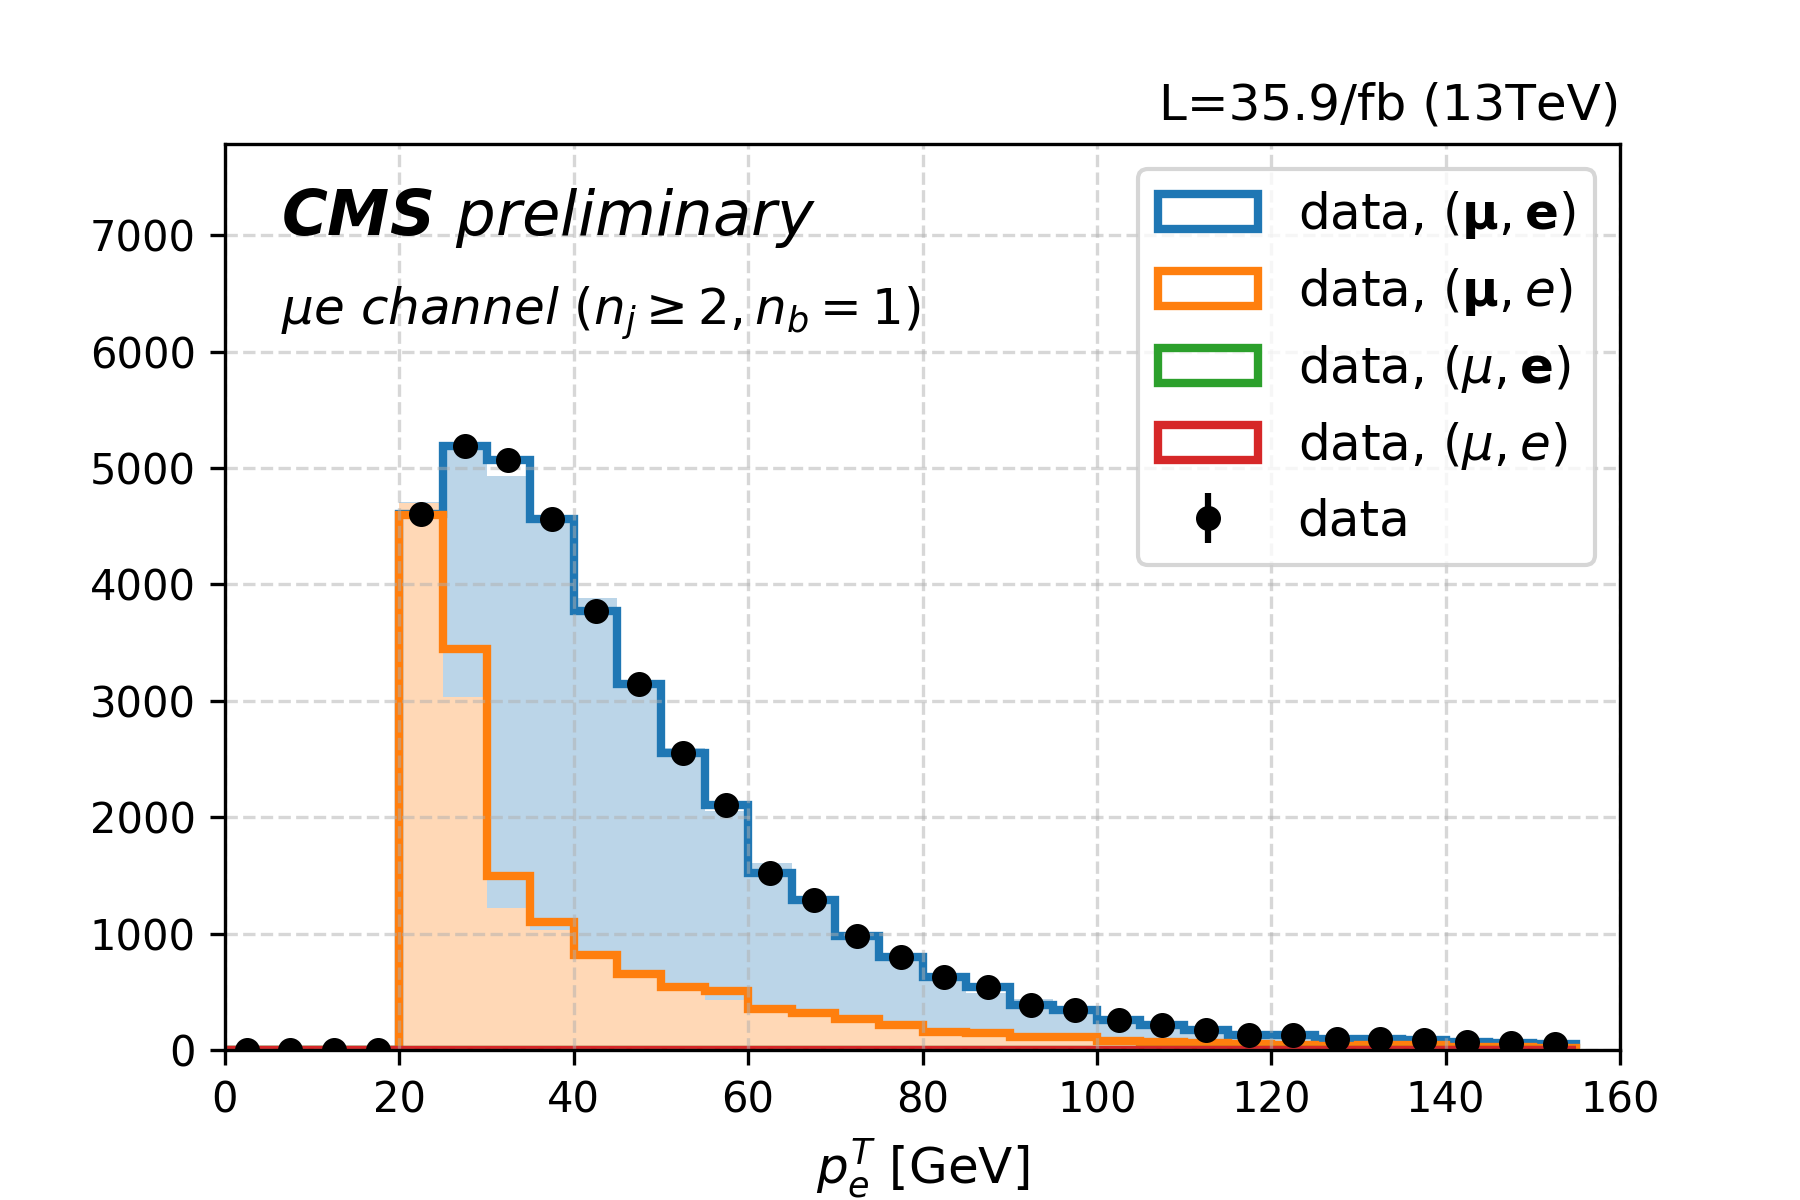
\includegraphics[width=0.49\textwidth]{chapters/Analysis/sectionSelection/figures/trgLep_emu.png}
    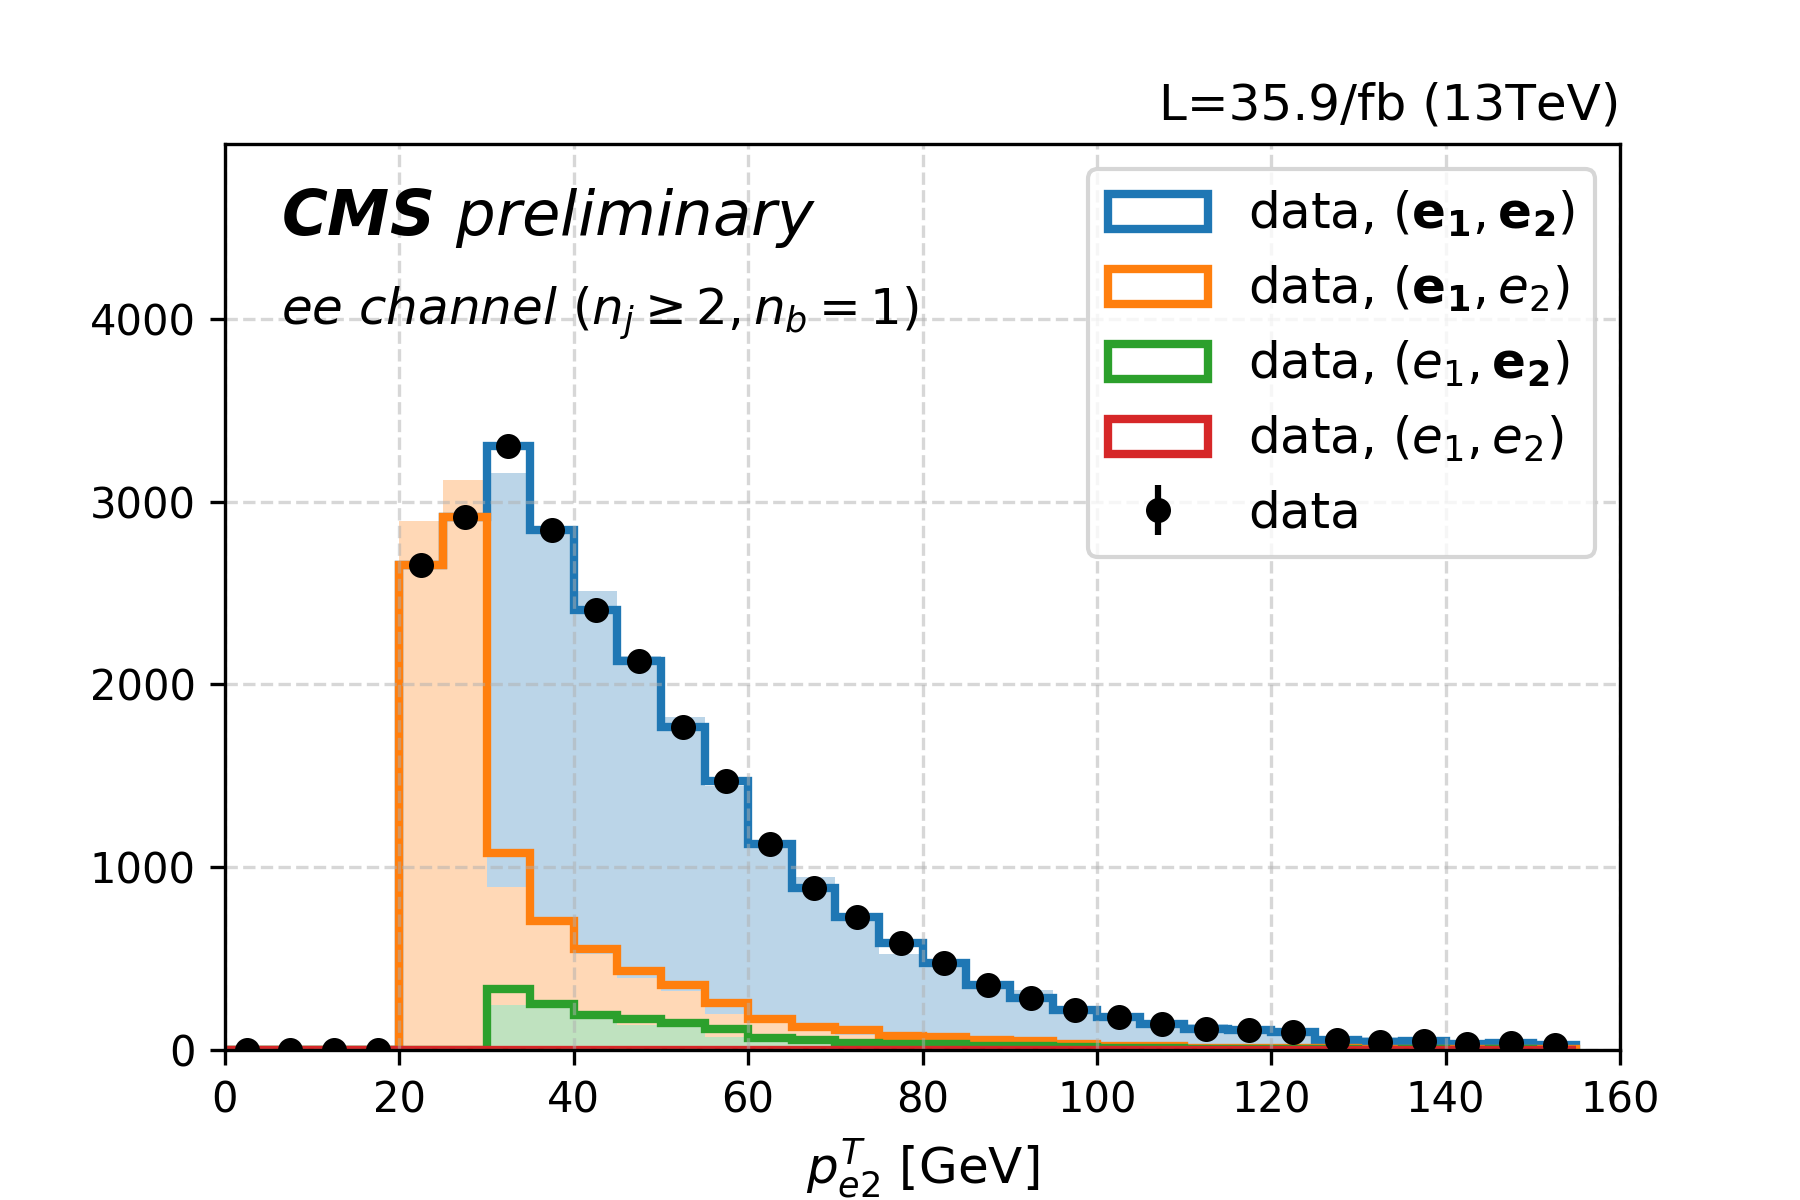
\includegraphics[width=0.49\textwidth]{chapters/Analysis/sectionSelection/figures/trgLep_ee.png}
    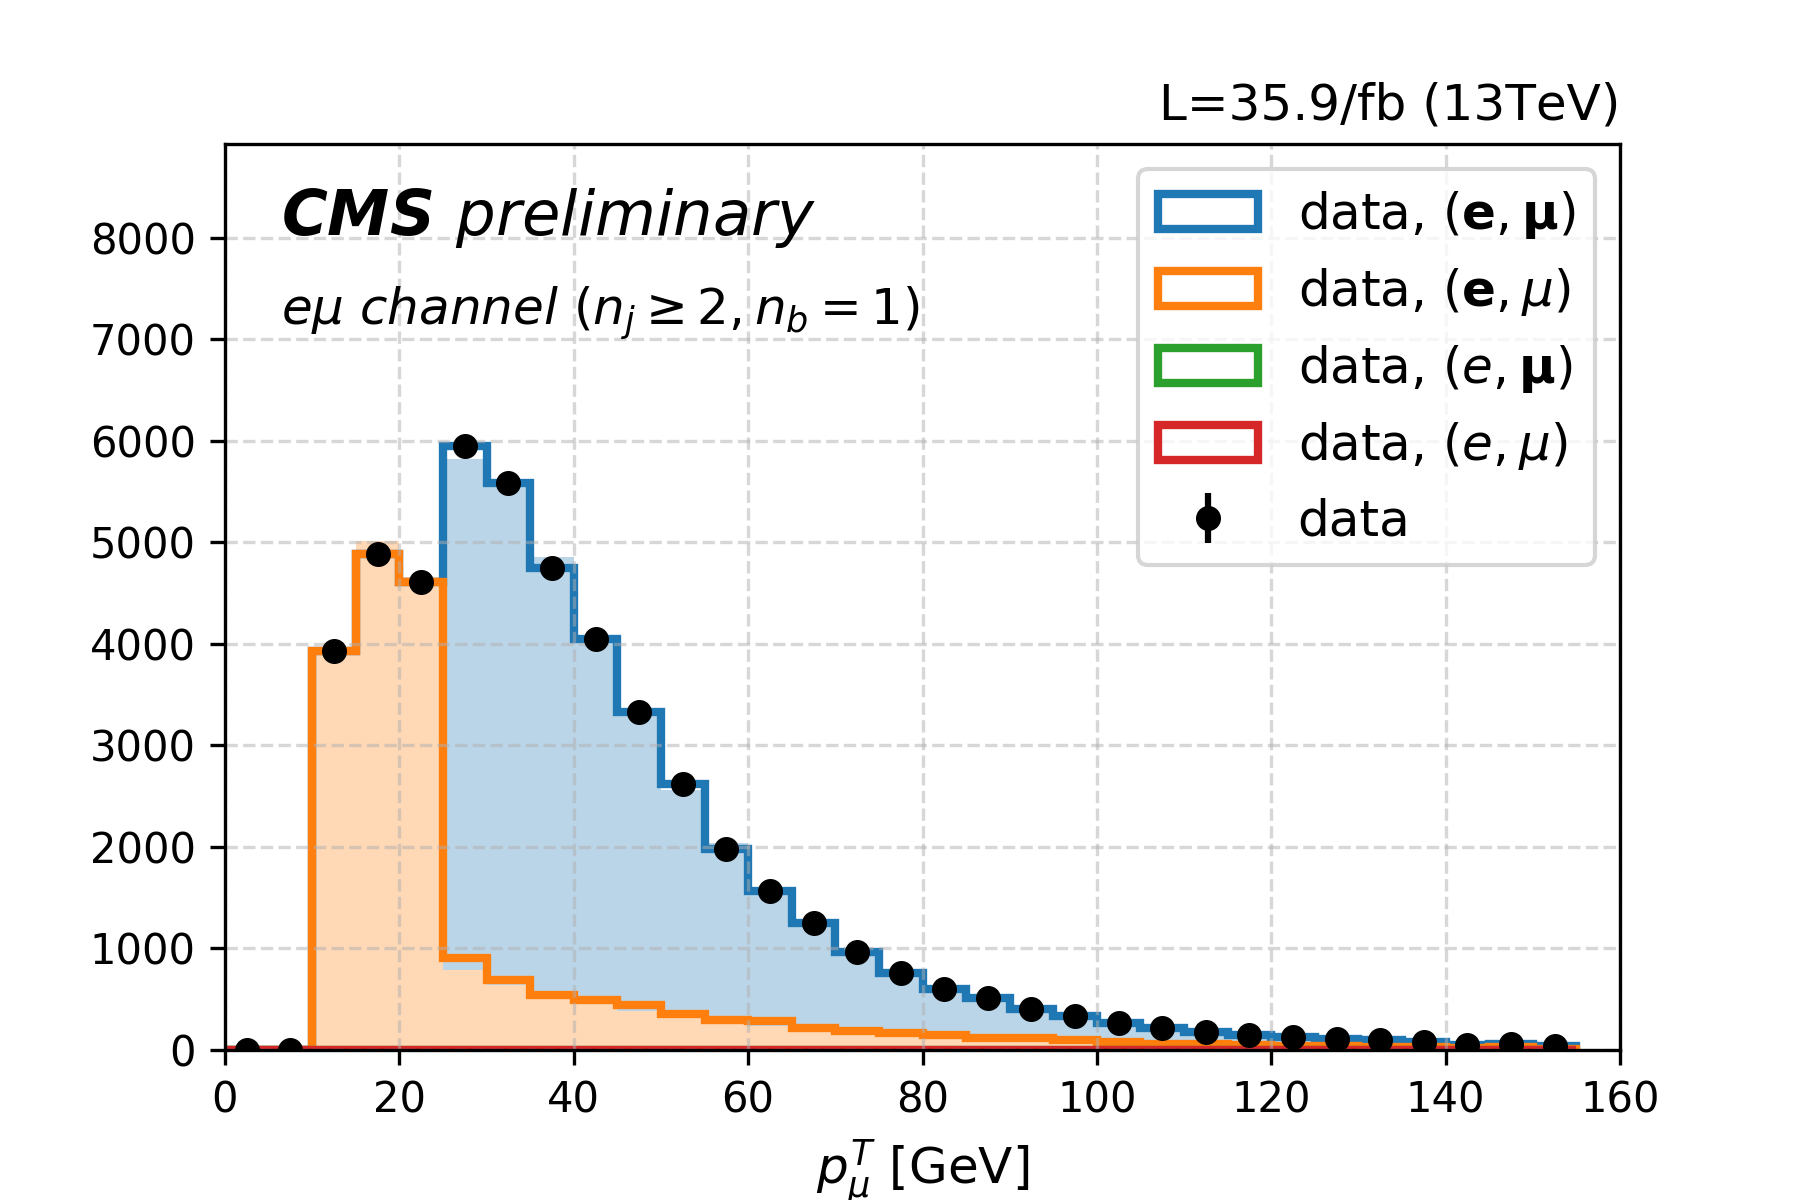
\includegraphics[width=0.49\textwidth]{chapters/Analysis/sectionSelection/figures/trgLep_emu2.png}
    \caption{caption}
    \label{fig:analysis:selection:trigger}
\end{figure}


For the counting analysis, there is always a requirement that there be at least two jets and at least one b tagged jet. The categories are partitioned based on whether there is exactly one b jet or there are two or more b jets.  Additionally, the $e\mu$ selection is split into muon triggered and electron triggered categories: if the muon has the highest \pt and the muon trigger has fired it categorized as a $\mu e$ event; if the electron has highest \pt and the electron trigger fired it is categorized as an $e \mu$ event.

\begin{sidewaystable}[ht]
    \centering
    % \rule{1.5\textwidth}{0.8\textwidth}
    % \toprule
    \setlength{\tabcolsep}{0.0em}
    \renewcommand{\arraystretch}{2}
    \footnotesize
    \begin{tabular}{l|cccccccc|cc}
    \hline
        & QCD & VV  & $\gamma$ & Z & W & t & tW & tt & total & data      \\
    \hline
    
    $\mu e$, $n_b=1$                   &       --$\pm$     -- &     90.3$\pm$    4.2 &      0.9$\pm$    0.9 &    202.7$\pm$   37.6 &     13.4$\pm$    5.1 &      9.5$\pm$    2.6 &   2107.6$\pm$   53.1 &  38871.4$\pm$   87.5 &  41295.8$\pm$  109.2 &  41047.0$\pm$  202.6 \\ 
    $\mu e$, $n_b\geq2$                &       --$\pm$     -- &      5.9$\pm$    1.0 &       --$\pm$     -- &       --$\pm$     -- &      3.1$\pm$    2.2 &      2.3$\pm$    1.6 &    625.7$\pm$   28.9 &  22647.7$\pm$   66.8 &  23270.9$\pm$   74.1 &  23918.0$\pm$  154.7 \\ 
    \hline
    $\mu\mu$, $n_b=1$                  &       --$\pm$     -- &    370.4$\pm$    5.8 &      4.1$\pm$    1.8 &  18046.9$\pm$  455.4 &     52.4$\pm$   11.7 &     55.8$\pm$    6.7 &   3406.2$\pm$   68.8 &  62266.6$\pm$  112.4 &  84202.3$\pm$  474.3 &  84284.0$\pm$  290.3 \\ 
    $\mu\mu$, $n_b\geq2$               &       --$\pm$     -- &     45.8$\pm$    1.5 &      0.0$\pm$    0.0 &   1945.7$\pm$  142.0 &      3.6$\pm$    2.6 &      3.9$\pm$    1.8 &    959.3$\pm$   36.2 &  35685.2$\pm$   85.1 &  38643.4$\pm$  169.6 &  39253.0$\pm$  198.1 \\ 
    \hline
    $\mu\tau$, $n_b=1$                 &   1130.7$\pm$  108.8 &     52.3$\pm$    2.6 &     11.8$\pm$    3.2 &    866.7$\pm$   78.7 &    730.8$\pm$   42.9 &    182.6$\pm$   12.4 &   1291.0$\pm$   41.9 &  18430.0$\pm$   60.6 &  22695.9$\pm$  159.6 &  21621.0$\pm$  147.0 \\ 
    $\mu\tau$, $n_b\geq2$              &    346.6$\pm$   51.5 &      5.5$\pm$    0.7 &      0.9$\pm$    0.8 &    103.6$\pm$   29.6 &     56.9$\pm$   14.4 &     36.8$\pm$    5.6 &    322.6$\pm$   21.0 &   9647.6$\pm$   43.7 &  10520.4$\pm$   78.3 &   9934.0$\pm$   99.7 \\ 
    \hline
    $\mu$+jets, $n_b=1$                &  24300.4$\pm$ 3404.9 &    371.0$\pm$    5.2 &   1501.2$\pm$   67.5 &   7533.2$\pm$  265.9 &  49248.1$\pm$  327.3 &   8484.6$\pm$   85.3 &  24447.8$\pm$  187.0 & 514064.6$\pm$  327.2 & 629950.9$\pm$ 3453.3 & 630704.0$\pm$  794.2 \\ 
    $\mu$+jets, $n_b\geq2$             &   4650.7$\pm$ 1399.5 &     61.4$\pm$    2.0 &    248.3$\pm$   31.8 &   1331.9$\pm$  114.0 &   6524.2$\pm$  118.8 &   5172.2$\pm$   66.7 &  10335.6$\pm$  121.4 & 356185.1$\pm$  272.2 & 384509.5$\pm$ 1442.2 & 385397.0$\pm$  620.8 \\ 
    \hline
    $e e$, $n_b=1$                     &       --$\pm$     -- &    138.2$\pm$    3.6 &      2.8$\pm$    1.2 &   4726.5$\pm$  215.7 &      5.4$\pm$    2.8 &      1.1$\pm$    0.8 &   1382.0$\pm$   42.7 &  23447.3$\pm$   66.9 &  29703.3$\pm$  229.9 &  29491.0$\pm$  171.7 \\ 
    $e e$, $n_b\geq2$                  &       --$\pm$     -- &     16.2$\pm$    0.9 &      0.1$\pm$    0.1 &    500.5$\pm$   67.8 &      3.7$\pm$    2.6 &      2.1$\pm$    1.2 &    371.4$\pm$   22.1 &  13412.7$\pm$   50.7 &  14306.6$\pm$   87.5 &  14334.0$\pm$  119.7 \\ 
    \hline
    $e\mu$, $n_b=1$                    &       --$\pm$     -- &    127.2$\pm$    4.9 &     25.5$\pm$   13.2 &    411.9$\pm$   52.7 &     32.8$\pm$    7.2 &     37.6$\pm$    5.4 &   2917.6$\pm$   62.7 &  49878.6$\pm$   99.2 &  53431.1$\pm$  129.8 &  52362.0$\pm$  228.8 \\ 
    $e\mu$, $n_b\geq2$                 &       --$\pm$     -- &      9.0$\pm$    1.3 &      1.9$\pm$    1.1 &     59.0$\pm$   19.5 &      6.5$\pm$    3.2 &      6.1$\pm$    2.2 &    837.9$\pm$   33.8 &  28374.1$\pm$   74.9 &  29294.5$\pm$   84.6 &  29860.0$\pm$  172.8 \\ 
    \hline
    $e\tau$, $n_b=1$                   &    874.2$\pm$   90.3 &     38.0$\pm$    2.1 &    194.5$\pm$   38.8 &    677.8$\pm$   69.3 &    456.3$\pm$   32.9 &    125.3$\pm$   10.0 &    908.2$\pm$   34.6 &  12884.7$\pm$   49.7 &  16159.1$\pm$  139.0 &  15309.0$\pm$  123.7 \\ 
    $e\tau$, $n_b\geq2$                &     94.2$\pm$   46.3 &      3.0$\pm$    0.4 &     10.0$\pm$    2.9 &     53.4$\pm$   21.3 &     28.7$\pm$    8.5 &     43.4$\pm$    6.0 &    196.1$\pm$   15.9 &   6682.4$\pm$   35.8 &   7111.3$\pm$   65.1 &   7006.0$\pm$   83.7 \\ 
    \hline
    $e$+jets, $n_b=1$                  &  25625.1$\pm$ 2941.3 &    494.9$\pm$    5.1 &  12035.7$\pm$  173.0 &  13119.8$\pm$  323.2 &  34481.3$\pm$  266.1 &   5786.3$\pm$   68.8 &  17454.7$\pm$  154.8 & 360917.6$\pm$  268.5 & 469915.4$\pm$ 2992.9 & 464543.0$\pm$  681.6 \\ 
    $e$+jets, $n_b\geq2$               &   3327.4$\pm$ 1476.4 &     84.5$\pm$    2.0 &   2095.3$\pm$   78.4 &   2520.8$\pm$  138.5 &   4696.3$\pm$   98.0 &   3524.2$\pm$   53.7 &   7616.3$\pm$  102.3 & 249557.0$\pm$  223.4 & 273421.8$\pm$ 1509.3 & 274162.0$\pm$  523.6 \\ 
    \hline

    \end{tabular}
    \caption{Estimates of the yields. The estimate of the expected yield is compared to
    the yield observed from data.  Uncertainties are statistical only.
    \label{tab:yields}}
\end{sidewaystable}

\begin{sidewaystable}[ht]
    \centering
    \setlength{\tabcolsep}{0.4em}
    \renewcommand{\arraystretch}{1.5}

    \caption{Composition of accepted $t\bar{t}$+$tW$ events, breakdown by 21 WW decay.  Values are in percent.}
    \resizebox{\textwidth}{!}{
    \begin{tabular}{|l|cc|cc|cc|cc|cc|cc|cc|cc|}
    
    
    \hline
    channel & \multicolumn{2}{|c|}{$\mu e$} & \multicolumn{2}{c|}{$\mu\mu$} & \multicolumn{2}{|c|}{$\mu \tau$} & \multicolumn{2}{|c|}{$\mu$+jets} & \multicolumn{2}{|c|}{$ee$} & \multicolumn{2}{|c|}{$e\mu$} & \multicolumn{2}{|c|}{$e \tau$} & \multicolumn{2}{|c|}{$e+jets$} \\
    \hline
    $\rm n_{b tag}$ & $n_b=1$ & $n_b\geq2$ & $n_b=1$ & $n_b\geq2$ & $n_b=1$ & $n_b\geq2$ & $n_b=1$ & $n_b\geq2$ & $n_b=1$ & $n_b\geq2$ & $n_b=1$ & $n_b\geq2$ & $n_b=1$ & $n_b\geq2$ & $n_b=1$ & $n_b\geq2$ \\ 
    \hline
    
    $tt/tW \to ee$                     &   -- &   -- &   -- &   -- &   -- &   -- &   -- &   -- & 87.4 & 87.8 &   -- &   -- &  0.7 &   -- &  3.1 &  3.1 \\ 
    $tt/tW \to \mu\mu$                 &   -- &   -- & 81.6 & 83.0 &   -- &   -- &  1.3 &  1.2 &   -- &   -- &   -- &   -- &   -- &   -- &   -- &   -- \\ 
    $tt/tW \to e\mu$                   & 86.5 & 87.0 &   -- &   -- &  0.8 &  0.5 &  3.3 &  3.3 &   -- &   -- & 82.7 & 84.1 &   -- &   -- &  1.4 &  1.4 \\ 
    $tt/tW \to \tau_{e}\tau_{e}$       &   -- &   -- &   -- &   -- &   -- &   -- &   -- &   -- &   -- &   -- &   -- &   -- &   -- &   -- &   -- &   -- \\ 
    $tt/tW \to \tau_{\mu}\tau_{\mu}$   &   -- &   -- &  0.7 &  0.6 &   -- &   -- &   -- &   -- &   -- &   -- &   -- &   -- &   -- &   -- &   -- &   -- \\ 
    $tt/tW \to \tau_{e}\tau_{\mu}$     &   -- &   -- &   -- &   -- &   -- &   -- &   -- &   -- &   -- &   -- &  0.6 &  0.6 &   -- &   -- &   -- &   -- \\ 
    $tt/tW \to \tau_{e}\tau_{h}$       &   -- &   -- &   -- &   -- &   -- &   -- &   -- &   -- &   -- &   -- &   -- &   -- &  3.1 &  3.2 &   -- &   -- \\ 
    $tt/tW \to \tau_{\mu}\tau_{h}$     &   -- &   -- &   -- &   -- &  3.2 &  3.6 &   -- &   -- &   -- &   -- &   -- &   -- &   -- &   -- &   -- &   -- \\ 
    $tt/tW \to \tau_{h}\tau_{h}$       &   -- &   -- &   -- &   -- &   -- &   -- &   -- &   -- &   -- &   -- &   -- &   -- &   -- &   -- &   -- &   -- \\ 
    $tt/tW \to e\tau_{e}$              &   -- &   -- &   -- &   -- &   -- &   -- &   -- &   -- & 11.7 & 11.5 &   -- &   -- &   -- &   -- &  0.8 &  0.8 \\ 
    $tt/tW \to e\tau_{\mu}$            &  4.1 &  4.0 &   -- &   -- &   -- &   -- &   -- &   -- &   -- &   -- & 11.2 & 11.0 &   -- &   -- &   -- &   -- \\ 
    $tt/tW \to e\tau_{h}$              &   -- &   -- &   -- &   -- &   -- &   -- &   -- &   -- &   -- &   -- &   -- &   -- & 57.5 & 63.6 &  3.4 &  3.6 \\ 
    $tt/tW \to \mu\tau_{e}$            &  8.3 &  8.2 &   -- &   -- &   -- &   -- &  0.6 &  0.7 &   -- &   -- &  3.6 &  3.6 &   -- &   -- &   -- &   -- \\ 
    $tt/tW \to \mu\tau_{\mu}$          &   -- &   -- & 15.7 & 15.8 &   -- &   -- &   -- &   -- &   -- &   -- &   -- &   -- &   -- &   -- &   -- &   -- \\ 
    $tt/tW \to \mu\tau_{h}$            &   -- &   -- &   -- &   -- & 57.4 & 63.6 &  3.4 &  3.6 &   -- &   -- &   -- &   -- &   -- &   -- &   -- &   -- \\ 
    $tt/tW \to eh$                     &   -- &   -- &   -- &   -- &   -- &   -- &   -- &   -- &   -- &   -- &  1.6 &   -- & 35.9 & 30.5 & 85.6 & 85.4 \\ 
    $tt/tW \to \mu h$                  &   -- &   -- &  1.7 &  0.5 & 35.7 & 30.1 & 85.3 & 85.3 &   -- &   -- &   -- &   -- &   -- &   -- &   -- &   -- \\ 
    $tt/tW \to \tau_{e}h$              &   -- &   -- &   -- &   -- &   -- &   -- &   -- &   -- &   -- &   -- &   -- &   -- &  1.9 &  1.6 &  4.8 &  4.7 \\ 
    $tt/tW \to \tau_{\mu}h$            &   -- &   -- &   -- &   -- &  2.1 &  1.6 &  5.0 &  4.9 &   -- &   -- &   -- &   -- &   -- &   -- &   -- &   -- \\ 
    $tt/tW \to \tau_{h}h$              &   -- &   -- &   -- &   -- &   -- &   -- &   -- &   -- &   -- &   -- &   -- &   -- &   -- &   -- &   -- &   -- \\ 
    $tt/tW \to hh$                     &   -- &   -- &   -- &   -- &   -- &   -- &   -- &   -- &   -- &   -- &   -- &   -- &   -- &   -- &   -- &   -- \\ 

    \hline
    \end{tabular}}
    \label{tab:analysis:selection:signal_breakdown}
    
\end{sidewaystable}


\FloatBarrier


